\documentclass{article}
\def\name{Suruz Miah}
\def\coursetitle{Electrical Engineering Fundamentals Laboratory}
\def\dept{Electrical and Computer Engineering Department}
\def\college{Caterpillar College of Engineering and Technology}
\def\uname{Bradley University}





\def\labTitle{Experiment 14: Introduction to Embedded Computer}



%%% set paper margins
\oddsidemargin=-0.2in % -.3 for a4 paper
\evensidemargin=.5in
\textwidth=7.0in
\topmargin=-.4in
\textheight=9.0in
\parindent=.2in
\newcommand{\vsmallskip}[0]{}
\newcommand{\midskip}[0]{\vspace{3mm}}

% Customize page headers
\usepackage{fancyhdr,lastpage}
\usepackage{hyperref}
\hypersetup{
    colorlinks=true,       % false: boxed links; true: colored links
    linkcolor=blue,          % color of internal links
    citecolor=red,        % color of links to bibliography
    filecolor=magenta,      % color of file links
    urlcolor=blue           % color of external links
}
\usepackage{amsmath,amssymb,bm,mathrsfs}
\usepackage{mathtools}
\usepackage{graphicx}
\usepackage{caption}
\usepackage{subfigure}
\usepackage[table,usenames,dvipsnames]{xcolor}
\usepackage{setspace}
%\doublespacing
\onehalfspacing
\usepackage{array} % related to table
\usepackage{float}
\usepackage{verbatim}
\usepackage{epstopdf}
\usepackage{booktabs}
\epstopdfsetup{suffix={}}
\usepackage{siunitx}
\sisetup{unitsep = \cdot}
\usepackage{tikz}
\usepackage[siunitx]{circuitikz}
\def\myCktGrid{0.5}



\usepackage{todonotes}
\usepackage{enumerate}

\newtheorem{example}{Example}
\newtheorem{exercise}{Exercise}
\newtheorem{definition}{Definition}

\usepackage{tikz} % tikz's drawing pad's gridsize = 1cm
\usetikzlibrary{circuits.logic.US,circuits.logic.IEC}


% \usepackage[framemethod=tikz]{mdframed}
% \mdfsetup{%
% backgroundcolor=red!10,
% roundcorner=0pt}

%%%% Design your own mdframe box
\usepackage[framemethod=TikZ]{mdframed}
\newcounter{prelab}\setcounter{prelab}{0}
\renewcommand{\theprelab}{~\#\arabic{prelab}}
\newenvironment{prelab}[2][]{%
    \refstepcounter{prelab}
 
    % Code for box design goes here.
\ifstrempty{#1}%
% if condition (without title)
{\mdfsetup{%
    frametitle={%
        \tikz[baseline=(current bounding box.east),outer sep=0pt]
        \node[anchor=east,rectangle,fill=blue!20]
        {\strut Prelab~\theprelab};}
    }%
% else condition (with title)
}{\mdfsetup{%
    frametitle={%
        \tikz[baseline=(current bounding box.east),outer sep=0pt]
        \node[anchor=east,rectangle,fill=blue!20]
        {\strut Prelab~\theprelab:~#1};}%
    }%
}%
% Both conditions
\mdfsetup{%
    innertopmargin=10pt,linecolor=blue!20,%
    linewidth=0.1pt,topline=true,%
    frametitleaboveskip=\dimexpr-\ht\strutbox\relax%
}
 
\begin{mdframed}[backgroundcolor=yellow!5, roundcorner=10pt,outerlinecolor= blue!70!black,outerlinewidth=1.2]\relax}{%
\end{mdframed}}




%\pagestyle{fancy}

%\rfoot{\date{\today}}
\lhead{S.~Miah}
% \chead{\coursecode:~\coursetitle}
\rhead{\uname}

\renewcommand{\headrulewidth}{1.5pt}
\renewcommand{\footrulewidth}{0.4pt}

\cfoot{%\hspace{\footpageshift}%
       \parbox{4in}{\, \hfill Page~ %
                    \arabic{page} of \protect\pageref*{LastPage} % +LP
%                    \arabic{page}                               % -LP
                    \hfill \,}}
\lfoot{ECE Department}   % header at lower left corner
% \rfoot{\labNumber}   % header at lower right corner

%\renewcommand{\thefootnote}{$\star$} 

\begin{document}

\centerline{\href{http://www.bradley.edu}{
\includegraphics[height=0.5in]{figs/logoBU1-Print}}}

\begin{center}
\vspace*{1.0cm}
{\bf \LARGE %
  Mechatronics Laboratory Experiments}

% \vspace*{1.0cm}

% {\Large
% \semester
% }

\vspace*{2.0cm}

{\color{BrickRed}
\hrule height 1.5pt
\midskip
}
%\hrulefill\\
{\LARGE %\labNumber: 
\labTitle%~\footnote{This lab task is adapted from reference~\cite{Buchla2010}}%
}\\
\midskip
{\color{BrickRed}
\hrule height 1.5pt
\midskip
}
%\hrulefill\\
\vspace*{0.15cm}
\begin{flushright}
{\Large
Dr.~\href{http://personalpages.bradley.edu/~smiah}{Suruz \textsc{Miah}}
%Dr.~\href{http://personalpages.bradley.edu/~smiah}{Suruz \textsc{Miah}} and  \href{mailto:aferrebee@mail.bradley.edu}{Alex Ferrebee}
}
\end{flushright}

\vspace*{1.0cm}
\noindent
~\hfill\boxed{\textbf{Total: 100 points}}


\end{center}

\vspace*{1.0cm}
\section*{\textit{Notes}}
\begin{itemize}
\item Individual group work only. 
  % \item Only electronic submissions through Sakai will be accepted.
  
\item See the ``Deliverables'' section of this document for submission guideline. 

\item Pay attention to the due date. %$10$ points penalty will be applied for each day of delay. 
\item All students should be be aware of the regulations of the Bradley University's Breach of Academic Integrity at \url{http://www.bradley.edu/academic/undergradcat/20142015/overview-archeating.dot}
\end{itemize}


\begin{center}
\vspace*{2.0cm}
\dept\\
\college\\
\href{http://www.bradley.edu/}{\uname}
\end{center}
\thispagestyle{empty}
\newpage


%\date{ }
%\maketitle
%
%\thispagestyle{fancy} % shows header and footer on all the  pages (including first page)
%\thispagestyle{empty}
\pagestyle{fancy}
%\renewcommand{\contentsname}{ }
% % if you want to include table of contents
% 1. Replace ``section*{'' by ``section{'' in ``research-uottawa.tex'' and ``teaching-uottawa.tex''
% 2. Activate the following two lines
 \renewcommand{\contentsname}{Table of Contents}
 \tableofcontents %Inhaltsverzeichnis
 

 %%%%%
 
The purpose of this laboratory work is to set up computational and experimental platforms using a single-board computer\footnote{The author would like to thank students (especially Eric Jones and Dakota Adra) of robotics and mechatronics group of ECE department for testing some laboratory experiments.}. There are several single-board computers available in the market. Here, a linux-enabled robotics computer will be utilized for conducting a set of laboratory experiments.

\section{Parts}
\label{sec:partsNeeded}
The following parts are required to conduct this laboratory experiment. %
%
\begin{enumerate}
% \item Breadboard,
\item BeagleBone Blue (BBBlue) single-board computer\footnote{\href{https://www.renaissancerobotics.com/BeagleboneBlue.html}{https://www.renaissancerobotics.com/BeagleboneBlue.html}}
\item 8/16/32 GB micro SD card
\item Micro-USB cable 
\item Laptop/desktop computer 
\end{enumerate}


\section{Hardware and Software}
A laptop computer (or desktop) with Windows 10 operating system installed is needed. In addition, a  BeagleBone Blue (BBBlue), which is a low-power open-source single-board, linux-enabled robotics computer is required. Figure~\ref{fig:BBBlue} depicts a BBBlue single-board computer showing its different  (external) hardware  interfacing slots and general purpose input/output (GPIO)  pins\footnote{\href{http://beagleboard.org/blue}{http://beagleboard.org/blue}}. %
%
\begin{figure}
    \centering
    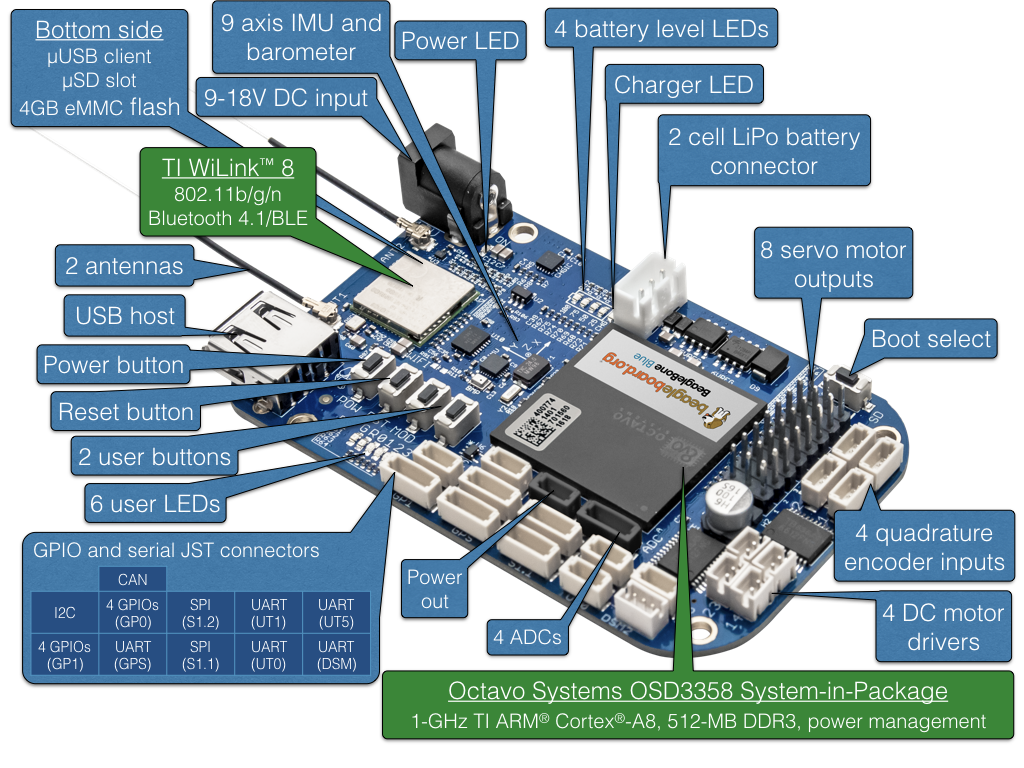
\includegraphics[width= 0.5\textwidth]{figs/img/Lab0/BeagleBone_Blue_balloons.png}
    \caption[BeagleBone Blue single-board computer.]{BeagleBone Blue single-board computer.}
    \label{fig:BBBlue}
\end{figure}
%
The BBBlue is to  be connected to a laptop computer running Windows 10 operating system using a micro-USB cable. The client software that need to be installed in the laptop are:  
\begin{enumerate}[a)]
    \item PuTTY,
    \item WinSCP, and 
    \item Etcher.
\end{enumerate}
%
These software are required to communicate with the BBBlue and to execute/access different files/folders of the BBBlue, which will be made clearer in the next section. 

\subsection{PuTTY}
\label{sec:putty}
PuTTY is an open-source client software that will be used to remotely communicate with a BBBlue from a local computer (laptop, for instance).  \hl{It is a terminal emulator, serial console and network file transfer application.}  PuTTY's Secure Shell (SSH) protocol is used to communicate between the Linux Shell (or console) in the local computer and the BBBlue. 

\begin{mdframed}[frametitle=Download and installation, backgroundcolor=yellow!5, roundcorner=7pt,outerlinecolor= blue!70!black,outerlinewidth=1.2]
  ``PuTTY" can be downloaded from \url{https://www.chiark.greenend.org.uk/~sgtatham/putty/latest.html} by clicking \emph{putty.exe}  (64-bit version) under the section labelled ``Alternative binary files." Save this file to your desktop.  Double click \emph{putty.exe} and follow the on-screen instructions to install it. 
\end{mdframed}


\subsection{WinSCP}
\label{sec:winSCP}
Similar to PuTTY, WinSCP (Windows Secure CoPy) is also a free and open-source  client software (for Microsoft Windows only) that is used to remotely communicate with the BBBlue from a laptop computer. The main function of WinSCP is the secure file transfer between a local (in this case, the laptop) and a remote (the BBBlue, for instance) computer.  In this laboratory work, WinSCP is used only to transfer files from a local computer directly into the remote directories on the BBBlue. %

\begin{mdframed}[frametitle=Download and installation, backgroundcolor=yellow!5, roundcorner=7pt,outerlinecolor= blue!70!black,outerlinewidth=1.2]
  To download WinSCP browse to ``WinSCP", go to \url{https://winscp.net/eng/download.php} and click on ``WinSCP::Official Site::Download". Then, download the most recent installation package (for example, \emph{WinSCP-5.11.3-setup.exe}, when this laboratory document was written) and save this file to your desktop. Double-click on the executable file \emph{WinSCP-5.11.3-setup.exe} and follow the on-screen instructions to install it. In the installation process, select \emph{Typical Installation} then select the \emph{Commander Style}.
\end{mdframed}

\subsection{Etcher}
\label{sec:etcher}

Etcher\footnote{\href{https://etcher.io/}{https://etcher.io/}}  is  a powerful \emph{DiskImager} software that is used to flash an operating system (OS) image on to an SD card or an USB drive. It is important that this software is used to flash an OS image on to the  SD card mounted on a BBBlue. Etcher ensures that every-bite of data is written correctly and prevents  from accidentally writing files to local hard-drives. 

\begin{mdframed}[frametitle=Download and installation, backgroundcolor=yellow!5, roundcorner=7pt,outerlinecolor= blue!70!black,outerlinewidth=1.2]
  Download Etcher software (e.g., \emph{Etcher-Setup-1.2.1-x64.exe}) from \url{https://etcher.io/}. Then, double-click \emph{Etcher-Setup-1.2.1-x64.exe} to install the Etcher application. 
\end{mdframed}




\section{Installing Operating System}
This section will focus on how to install a linux operating system on to a BBBlue single-board computer. The two main steps that need to be followed are:
\begin{enumerate}
    \item Flashing operating system (OS) on external memory card and 
    \item Flasing OS image on to BBBlue's built-in eMMC storage.
\end{enumerate}
%
These steps are briefly illustrated below. 
\subsection{Flashing OS Image on External Memory Card}
\label{sec:flashingOS}
% \subsection{Writing Debian Image to SD Card}
% \label{sec:writeImage2-SD-Card}

A unix-like operating system, Debian\footnote{\href{https://en.wikipedia.org/wiki/Debian}{https://en.wikipedia.org/wiki/Debian}}, image will be flashed on to an external memory card (SD card). If this is the first time you are connecting a BBBlue with the laptop, you will need to update the BBBlue with the latest operating system image. Follow the steps below\footnote{These steps are adapted from \url{http://beagleboard.org/getting-started}}:

\begin{enumerate}[a)]
  
\item Download the latest Debian\footnote{A computer operating system that is composed of free software} image from \url{https://beagleboard.org/latest-images}. It is recommended that you click \emph{Debian 9.5 2018-10-07 4GB SD IoT} to download the image \emph{bone-debian-9.5-iot-armhf-2018-10-07-4gb.img.xz}.   The IoT images provide more free disk space if you do not need to use a graphical user interface (GUI). Here, we will not be utilizing a GUI, so this IoT version is desired. 
\item Using 7-zip, unzip the downloaded software into a image folder (\emph{bone-debian-9.5-iot-armhf-2018-10-07-4gb.img}).

\item Insert a microSD card (minimum 8 GB) into SD card slot of your laptop. 
\item Run the Etcher application. A small window will appear. See Figure~\ref{fig:Etcher}. %
%
\begin{figure}
    \centering
    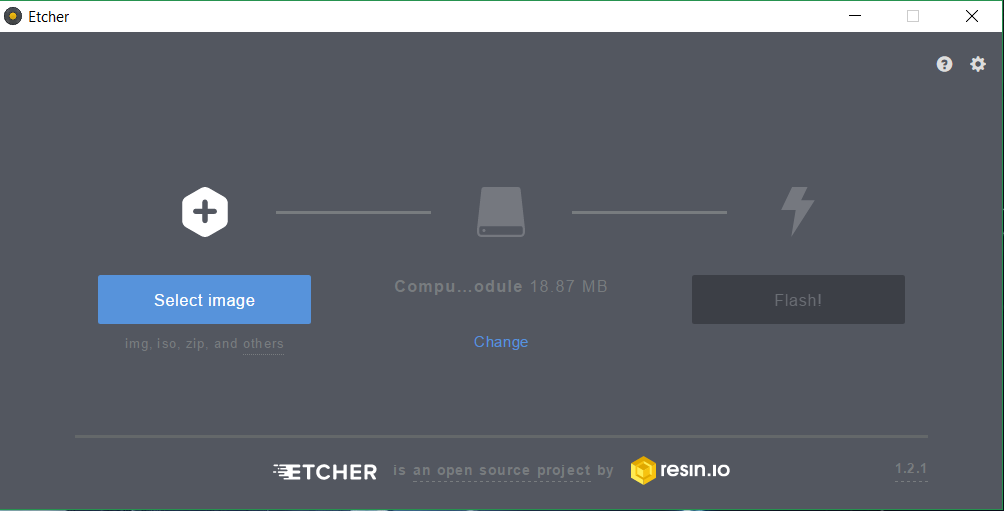
\includegraphics[width= 0.6\textwidth]{figs/img/Lab0/Etcher.png}
    \caption{Etcher application.}
    \label{fig:Etcher}
\end{figure}
%

\item Select the Debian image from where you saved it. Lastly, make sure that you select the correct file location for your SD card. Then press Flash, this may take  around five minutes (see Figures~\ref{fig:debianImageUpload},~\ref{fig:debianImageUploadSelectDrive},~and~\ref{fig:debianImageUploadSelectDriveFlashing}). 
%
\begin{figure}
    \centering
    \subfigure[][]{
    \label{fig:debianImageUpload}
    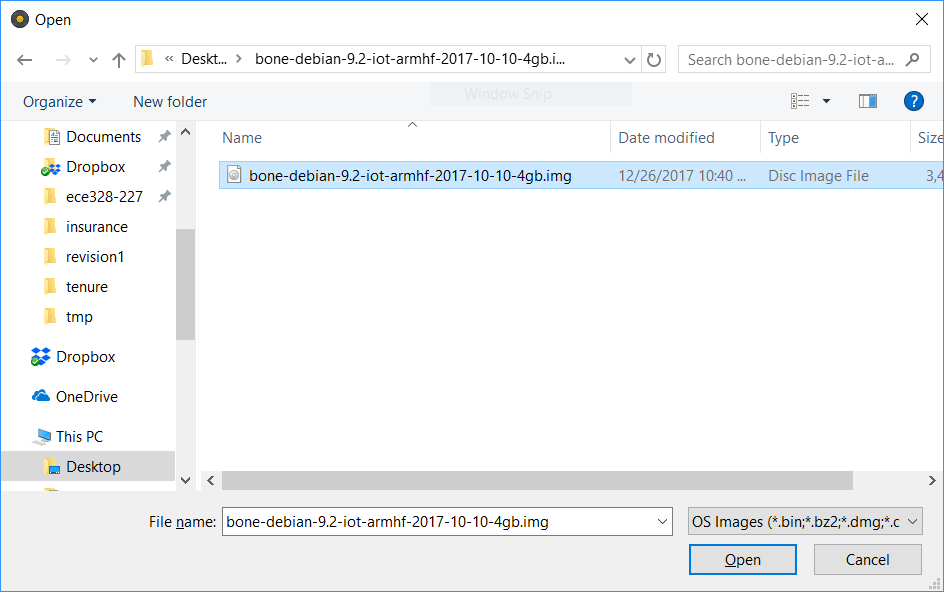
\includegraphics[width= 0.6\textwidth]{figs/img/Lab0/debianImageUpload}}
    \\
    \subfigure[][]{
    \label{fig:debianImageUploadSelectDrive}
    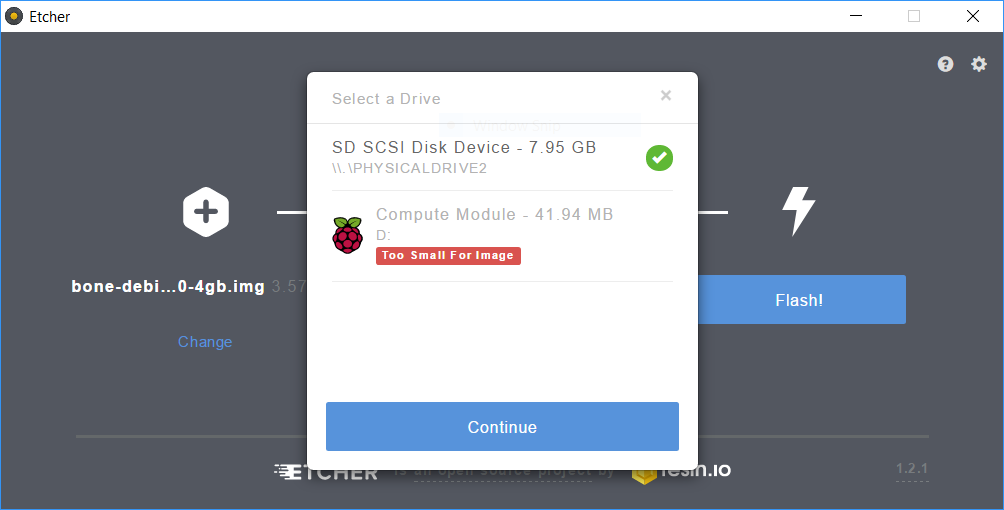
\includegraphics[width= 0.6\textwidth]{figs/img/Lab0/debianImageUploadSelectDrive}}    
    \\
    \subfigure[][]{
    \label{fig:debianImageUploadSelectDriveFlashing}
    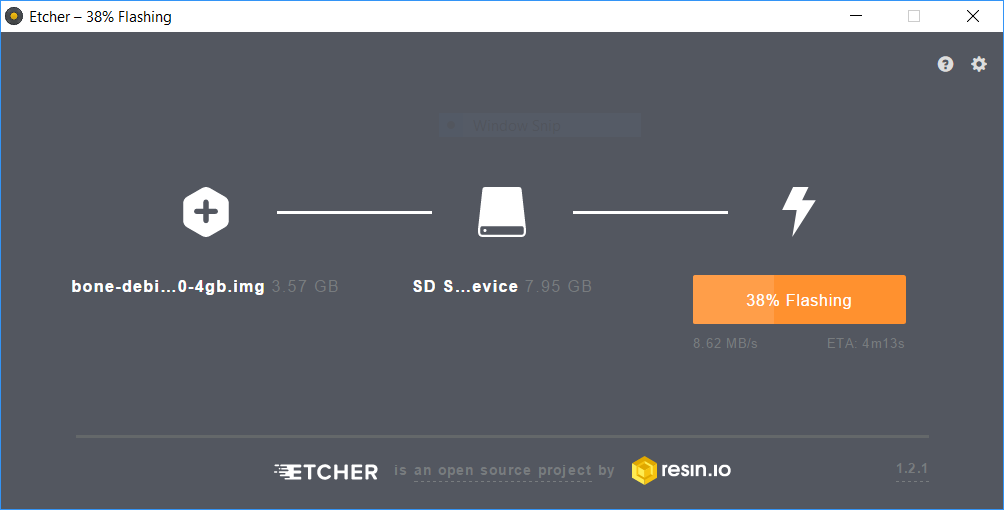
\includegraphics[width= 0.6\textwidth]{figs/img/Lab0/debianImageUploadSelectDriveFlashing}}
    \caption{\subref{fig:debianImageUpload} Selecting the image file,~\subref{fig:debianImageUploadSelectDrive} selecting drive of the microSD card, and~\subref{fig:debianImageUploadSelectDriveFlashing} flashing the image into the microSD card.}
    \label{fig:debianImageUpload2-MicroSD}
\end{figure}
%


\item When finished, you should see the Etcher window displaying \emph{Flash Complete!}. Safely eject the microSD card from your computer.
\end{enumerate}


\subsection{Flashing OS Image on to BBBlue's Built-In eMMC Storage}
It is recommended that BBBlue's built-in eMMC storage is flashed with the latest Debian OS image. For that, it is assumed that the latest Debian OS image is successfully written in the SD card following the instructions illustrated in the previous section. Then, follow the steps below\footnote{These instructions are adapted from \url{http://www.strawsondesign.com/docs/librobotcontrol/flashing.html}}.  

\begin{mdframed}[backgroundcolor=yellow!5, roundcorner=7pt,outerlinecolor= blue!70!black,outerlinewidth=1.2]
\begin{enumerate}[(a)]
    \item Make sure to power off BBBlue completely and insert the SD card with newly stored Debian OS image.
    \item Apply power through either USB or the DC power jack and watch the Blue USR LEDs. 
    \item BBBlue's USR LEDs should start blinking and then bouncing back and forth like a pong game. 
    \item When flashing the built-in eMMC is complete, all LEDs will stay on for a minute, and then turned off completely. 

\end{enumerate}
%
If you follow the above steps correctly, then flashing BBBlue's eMMC is complete. Make sure to remove the SD card to accidentally start the flashing process again.  Remove the BBBlue's micro-USB cable from your computer and reapply the power using the micor-USB cable by reconnecting it to the computer.


 Note that if the BBBlue is powered on with the SD card inserted and the USR LEDs do not blink in a regular pattern then it's possible the eMMC bootloader is old or somehow not configured to favor booting from the SD card automatically. In this case, insert the SD card into the (powered-down) BBBlue board, hold down the USER/BOOT button (denoted SD) and apply power, either by the USB cable or the DC power adapter. Release the button once all LEDs have turned on. After you have successfully booted up the board, LED0 will be blinking in a heartbeat pattern.
% Perhaps a way to check boot device.  
\end{mdframed}


\begin{mdframed}[frametitle=Testing OS with PuTTY, backgroundcolor=yellow!5, roundcorner=7pt,outerlinecolor= blue!70!black,outerlinewidth=1.2]
  \begin{itemize}
  \item Open PuTTY and type the IP address ``192.168.7.2'' in the ``Host Name (or IP address)'' box, ``22'' in the ``Port'' box, and then click ``Open''  (see Figure~\ref{fig:PuTTY-Configuration}). 
    
  \item Login as: ``debian'' with password: ``temppwd'' to see the console window similar to Figure~\ref{fig:PuTTY-Console}. 
  \end{itemize}
\end{mdframed}
%
\begin{figure}
  \centering
  \subfigure[][]{
    \label{fig:PuTTY-Configuration}
   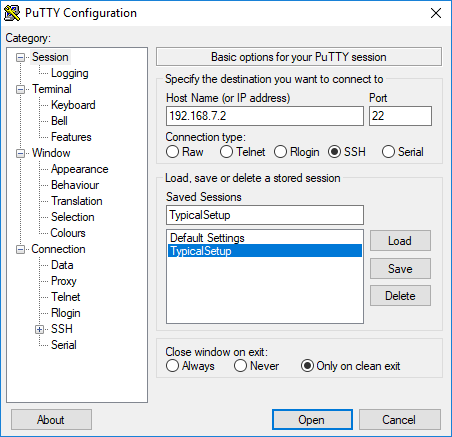
\includegraphics[width=0.3\textwidth,height=0.22\textheight]{figs/img/Lab0/PuTTY}
 }
   \subfigure[][]{
    \label{fig:PuTTY-Console}
   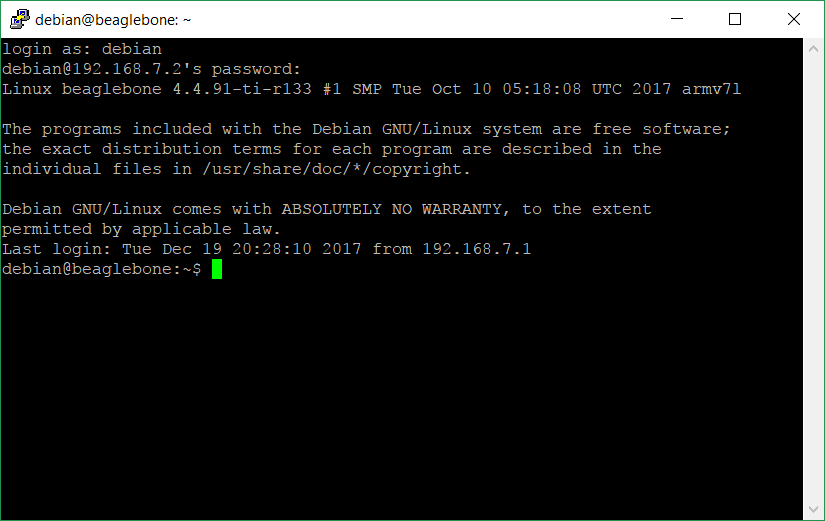
\includegraphics[width=0.5\textwidth,height=0.22\textheight]{figs/img/Lab0/PuTTY_Console}
 }
  \caption{\subref{fig:PuTTY-Configuration} PuTTY configuration and \subref{fig:PuTTY-Console} PuTTY console.}
  \label{fig:PuTTY1}
\end{figure}

\section{BBBlue Networking}
\label{sec:usbConn}
To download all necessary software for the BBBlue, it needs to first be connected with the internet. Experiments with a BBBlue will rely on the proper installation of device drivers and the latest version of Debian OS image installed. The previous section was focused on installing the latest Debian image on the to the BBBlue's built-in eMMC flash storage device. In this section, the main focus will be on how to connect BBBlue to the internet. For that, a proper driver for the laptop/desktop computer is to be installed.%

\subsection{Installing Drivers}
\label{sec:drivers}

To access BBBlue using USB connection,  
The drivers need to be installed for the operating system to give
network-over-USB access to the BBBlue. Note that drivers may not need to be
installed for computers operating Windows 10 or later. In case, the BBBlue is
not recognized with USB connection, follow the steps below to install the
driver. 

\begin{enumerate}[a)]
\item  Connect the BBBlue to the laptop/computer using the micro-USB cable. Once connected, the LEDs on the board will begin to light up. After the lights have flashed for a few seconds, LED0 will begin to light up in a heartbeat pattern. 

\item Go to windows \emph{File Explorer}
  
\item Scroll down and  click \emph{BeagleBone Getting Started} to see the window as shown in Figure~\ref{fig:BBBlue-Start}. %
  %
\begin{figure}
    \centering
    \boxed{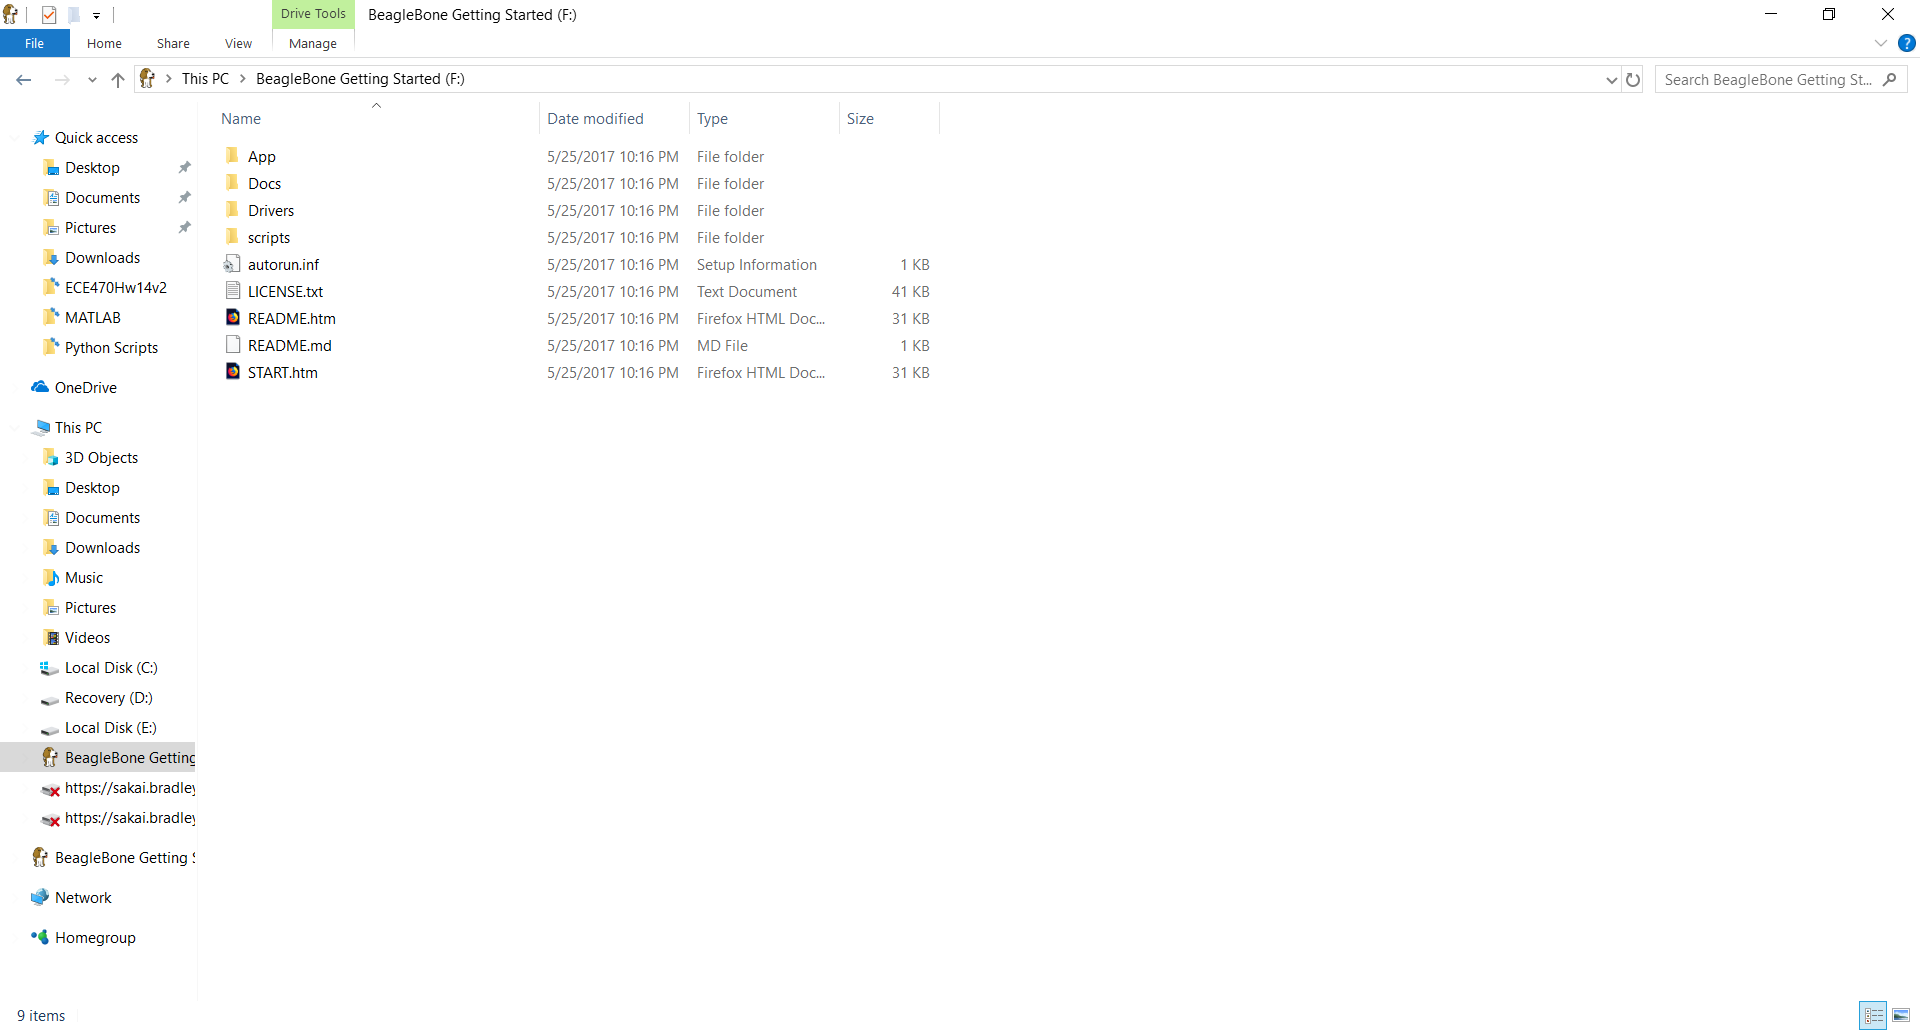
\includegraphics[width= 0.7\textwidth]{figs/img/Lab0/BBB_Start.png}}
    \caption{``BeagleBone Getting Started'' drive.}
    \label{fig:BBBlue-Start}
\end{figure}
%
\item Double-click on \emph{START.htm}.  It will take you to a web page %that will allow you to install the \underline{board drivers} for your operating system  to give network-over-USB access to the BBBlue. 
 %
\item Scroll down to \emph{\underline{Step \#2: Install drivers}} of the web page.  You will be given the option between a 32 and 64 bit BeagleBone Device Driver Installer: make sure you select the correct one for your system. For my case, I chose to click \emph{64-bit installer} and downloaded  and save the file \hl{\emph{BONE\_D64.exe}} on my desktop. 
% \begin{mdframed}[roundcorner = 5pt, backgroundcolor=yellow!20]
% \begin{verbatim}
% BONE_D64.exe
% \end{verbatim}
% \end{mdframed}
  
  \emph{\uppercase{\underline{do not install it yet}}.}

\end{enumerate}

The next steps will depend on your version of Windows OS. Here, we will assume you are using the Windows 10 operating system. %
%If you have Windows 7 or 8 please follow along with the instructional video in the provided link: \url{https://www.youtube.com/watch?v=b2_jS3ZMwtM}.\\ 
%Credit Jon Jellison/ram group youtube page? Include the timestamp!
% Note that this link explains how to ``Program in 'C'" and interface with the BeagleBone Black, however the process remains similar with the BeagleBone Blue.\\
% In the case of Windows 10 please follow the following steps:

\begin{enumerate}[a)]
    \item Press Windows button $\to$ click \emph{Settings} $\to$ click \emph{Update \& security} $\to$ \emph{Recovery}
    \item Once selected, you will see an \emph{Advanced startup} section appear on the right hand side $\to$ click \emph{Restart now}
    \item Once your Computer has rebooted, you will need to choose the \emph{Troubleshoot} option.
    \item Next, click on \emph{Advanced} options $\to$ click \emph{Startup Settings}.
    \item Here, you will be given a list of startup settings that you can change. The one we are looking for is \emph{Disable driver signature enforcement}. To choose this setting, you will need to press the F7 key.
    \item Since we are modifying boot time configuration settings, you will need to restart your computer one last time.
\end{enumerate}
Your computer believes that since these drivers are not digitally signed they are a threat to your computer. For this reason, we disable device driver signature enforcement. 


\begin{mdframed}[frametitle=Install BeagleBone Driver and Browse BeagleBone's webserver, backgroundcolor=yellow!5, roundcorner=7pt,outerlinecolor= blue!70!black,outerlinewidth=1.2]
  \begin{itemize}
  \item   Double-click \emph{BONE\_D64.exe} and follow the on-screen instructions. In case, the installation process is blocked due to windows security, make sure to choose \emph{Install this driver software anyway}. If drivers are installed properly, a window with all green check marks will be displayed as shown in Figure~\ref{fig:BBBlue-DriverInstalation}.
    
  \item To guarantee you are connected to the board, open a web browser and browse to ``http://192.168.7.2'' You should see a message:

    \emph{You board is connected!}\\
    \noindent BeagleBone running BoneScript 0.x.x at 192.168.7.2 

where ``0.x.x'' is the current version of the BoneScript. 
  \end{itemize}
  
\end{mdframed}

If there are issues browsing  ``http://192.168.7.2'', refer to Troubleshooting Problem \ref{trst:problem2}

  \begin{figure}
    \centering
    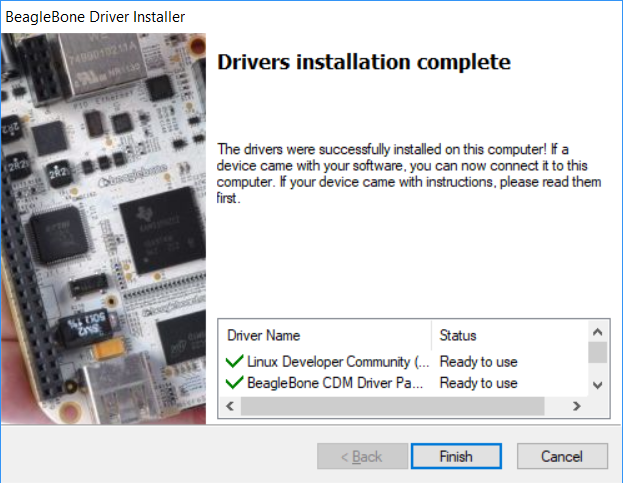
\includegraphics[scale=0.5]{figs/img/Lab0/BBB-DriverInstalation}
    \caption{BeagleBone driver installation complete.}
    \label{fig:BBBlue-DriverInstalation}
  \end{figure}
%
%===========================================================================================================
% http://beagleboard.org/getting-started#update
%===========================================================================================================

\subsection{File Transfer to BBBlue using WinSCP} \label{FileTransferWinSCP}
Files can be created and edited on the BBBlue through the terminal. However, sometimes it is more convenient to write a file on a laptop computer and then transfer the file to the BBBlue. This can be done using WinSCP client software that is installed in the laptop. To do that, follow the steps below. 
%
\begin{enumerate}
    \item Open WinSCP
    
    \item  To upload the file open WinSCP, enter hostname as ``192.168.7.2", port as ``22", username ``debian" and use the standard password ``temppwd" as shown in Figure~\ref{fig:winSCPlogin}. %
    %
    \begin{figure}
        \centering
        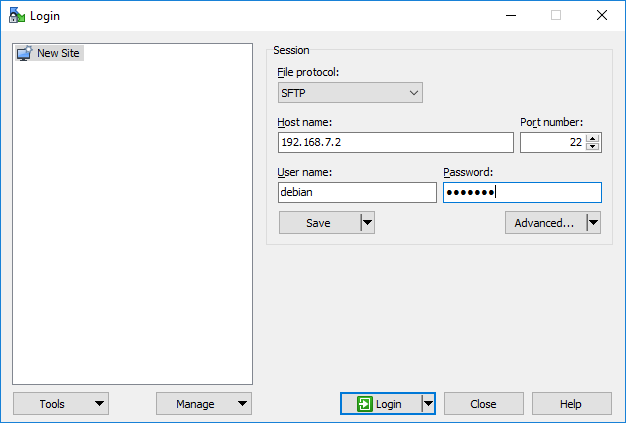
\includegraphics[width= 0.55\textwidth]{figs/img/Lab0/winSCP_login.png}
        \caption{Login BBBlue using WinSCP.}
        \label{fig:winSCPlogin}
    \end{figure}
    %
    
    \item You will now be presented with a double-pane window as shown in Figure~\ref{fig:winApp}. The left pane shows the content of the local directory and the right pan shows the content of the remote (in this case, BBBlue) directory. %
    \begin{figure}
        \centering
        % 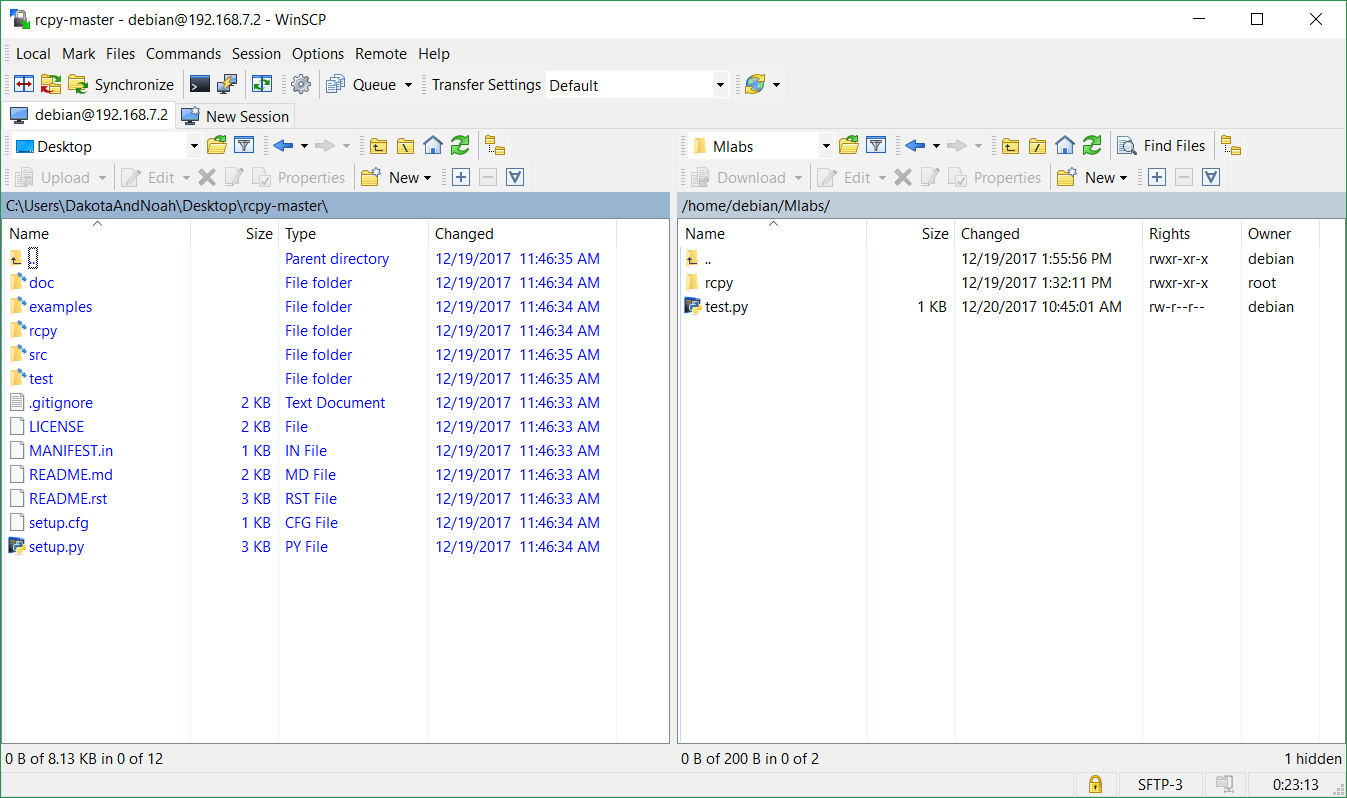
\includegraphics[width= 0.65\textwidth]{figs/img/Lab0/winSCP.png}
        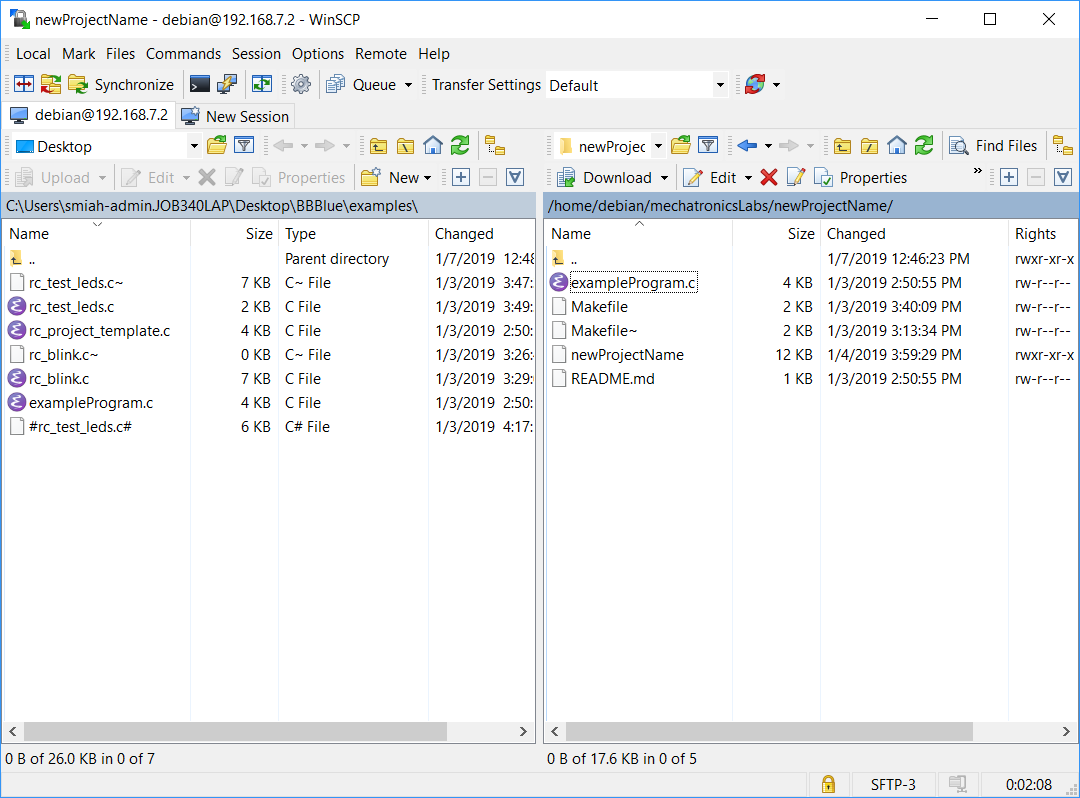
\includegraphics[width= 0.65\textwidth]{figs/img/Lab0/winSCP-C.PNG}        
        \caption{Transferring files using WinSCP application.}
        \label{fig:winApp}
    \end{figure}
    
    \item Select the program file \emph{exampleProgram.c} on the left pane (which is locally stored in your laptop), and then simply drag and drop in the remote directory (here, \emph{newProjectName/}) of the BBBlue as shown in the right pane of Figure~\ref{fig:winApp}. The file is now transferred to the BBBlue.%

    
\end{enumerate}

\subsection{Internet Connection}
Given that the driver software for BBBlue is installed properly in the computer
that is attached to the BBBlue, the focus is now to connect a BBBlue with the
internet using wifi. Depending on types of available wifi access points, the
BBBlue will be connected to the internet using two different methods. %
%
\begin{enumerate}
\item Connecting BBBlue with wifi using shared passkey
  
\item Connecting BBBlue with wifi using enterprise login  
\end{enumerate}

\subsubsection{Connecting BBBlue with Wifi using Shared Passkey}

In this section, we shall illustrate the procedure to connect a BBBlue with the
internet through the wifi network that is set up at home environment. Before
illustrating the steps below, make sure you have a reliable internet connection
through the home wifi network. Furthermore, it is assumed that the BBBlue is
connected to the computer through PuTTY console using 

\begin{verbatim}
 ssh debian@192.168.7.2
\end{verbatim}

with password ``temppwd'' with administrative privilege. Then, follow the steps
below.  

\begin{enumerate}[a)]
    \item Begin by typing 
         \begin{verbatim}
            ifconfig
         \end{verbatim}
         into the PuTTY interface. This will display the network configuration as shown in~\autoref{fig:ifconfig_1}. 
         
    \begin{figure}
        \centering
        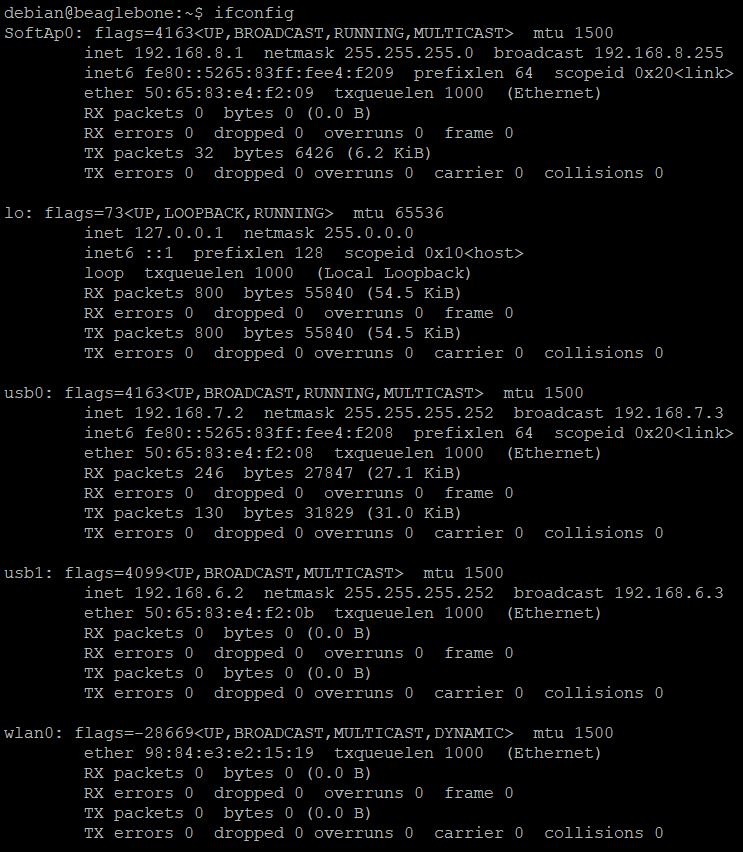
\includegraphics[width= 0.4\textwidth]{figs/img/Lab0/ifconfig_1.JPG}
        \caption{Displaying network status using \emph{ifconfig} command.}
        \label{fig:ifconfig_1}
    \end{figure} 

    \item As it can be seen from \autoref{fig:ifconfig_1}, in option \emph{wlan0:},
    \emph{RX packets 0 bytes 0 and TX packets 0 bytes 0.} This shows that there is
    no internet connection.

    
    \item The BBBlue will be connected to the internet using the application called
    ``connmanctl''. Therefore, key in the command
            \begin{verbatim}
                connmanctl
            \end{verbatim}
        to enter into the \emph{connmanctl} application.
    
    \item After entering the Connmanctl application, key in
        \begin{verbatim}
            enable wifi
        \end{verbatim}
    to ensure wireless capabilities are enabled on the BeagleBone.
    
    \item Next scan for possible wireless network connections by keying in
    \begin{verbatim}
        scan wifi
    \end{verbatim}
    The resulting output will display whether or not the scan was completed.
    \item Continue by keying in
    \begin{verbatim}
        services
    \end{verbatim}
    to display all scanned wireless networks.
    \item Next register all wireless networks by keying in
    \begin{verbatim}
        agent on
    \end{verbatim}
    Display should show that all agents were registered.
    
    \item Connect to wireless network by using passkey that corresponds to the network name ``BUother", for example: 
    \begin{verbatim}
        connect passkey
    \end{verbatim}
    where \textit{passkey} is the string  that corresponds to network name
    ``BUother", \textit{i.e.,} \emph{wifi\_9884e3$\ldots$} as shown in
    Figure~\ref{fig:connmanctl}. In case, the wifi network has a password, type
    the password when asked right after ``passphrase: WIFI\_PASSWORD'' 
    \item After connecting to the wireless network, key in the command
    \begin{verbatim}
        quit
    \end{verbatim}
    to leave the Connmanctl application. Refer to \autoref{fig:connmanctl} for an example of connecting to the internet.
    \begin{figure}[H]
        \centering
        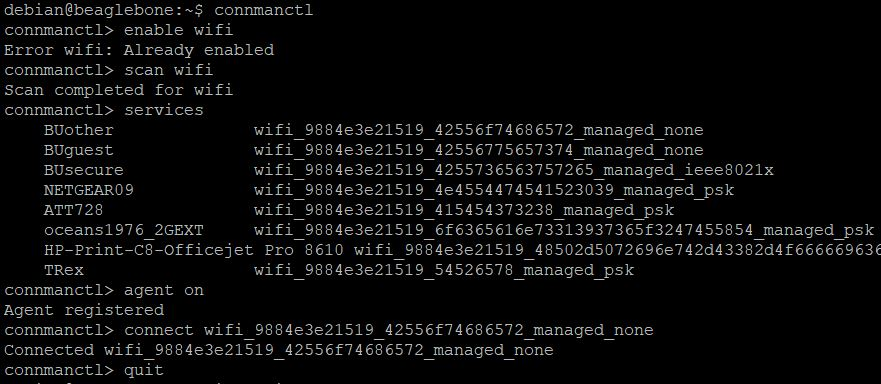
\includegraphics[width= 0.6\textwidth]{figs/img/Lab0/connmanctl.JPG}
        \caption{Connecting BBBlue to the  internet using passkey.}
        \label{fig:connmanctl}
    \end{figure}    
    \item You can now test the internet connection using a simple ping test to a web URL such as google.com:
    \begin{verbatim}
        ping www.google.com
    \end{verbatim}
%   
You should receive a positive response from the web URL server. Now that you are connected to the internet you can run updates and install any software as required.
\end{enumerate}


\subsubsection{Connecting BBBlue with Wifi using Enterprise Login}

In an office environment, such as university or enterprise, it is required to
use ``username'' followed by a password to connect to the internet through the
wifi network dedicated for the office. To connect the BBBlue to such a wifi
network, follow the steps below.

\begin{enumerate}[a)]
    \item Begin by typing 
         \begin{verbatim}
            ifconfig
         \end{verbatim}
         into the PuTTY interface. This will display the network configuration as shown in~\autoref{fig:ifconfig_1}.

\item As it can be seen from \autoref{fig:ifconfig_1}, in option \emph{wlan0:},
  \emph{RX packets 0 bytes 0 and TX packets 0 bytes 0.} This shows that there is
  no internet connection.

  
\item The application called ``connmanctl'' will be used to determine the name and SSID of the enterprise network. Therefore, key in the command
        \begin{verbatim}
            connmanctl
        \end{verbatim}
    to enter into the \emph{connmanctl} application.
    
    \item After entering the Connmanctl application, key in
        \begin{verbatim}
            enable wifi
        \end{verbatim}
    to ensure wireless capabilities are enabled on the BeagleBone.
    
    \item Next scan for possible wireless network connections by keying in
    \begin{verbatim}
        scan wifi
    \end{verbatim}
    The resulting output will display whether or not the scan was completed.
    \item Continue by keying in
    \begin{verbatim}
        services
    \end{verbatim}
    to display all scanned wireless networks as shown in \autoref{fig:wifi_services}. Note that the network BUsecure has a network ID that ends with ``ieee8021x.'' This indicates that the network uses Network Access Control instead of just a passkey.

    \begin{figure}
        \centering
        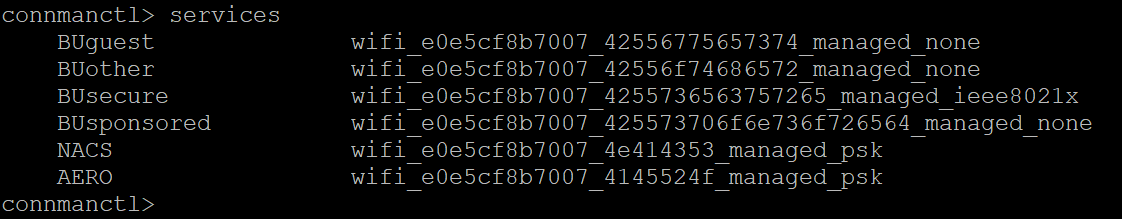
\includegraphics[width= 0.6\textwidth]{figs/img/Lab0/wifi_services.png}
        \caption{Listing available networks using \emph{services} command.}
        \label{fig:wifi_services}
    \end{figure}

    \item Key in the command
    \begin{verbatim}
        quit
    \end{verbatim}
    to leave the Connmanctl application.

    \item To connect the BBBlue to the enterprise network, a new file must be created in the \emph{/var/lib/connman} directory. This file can be created using a text editor such as Nano on the BBBlue, or it can be created on the laptop computer and transferred using WinSCP (see \ref{FileTransferWinSCP}). The filename should be the ID of the network with an extension of ``.config'' (\emph{wifi\_e0e5cf8b02c6\_4255736563757265\_managed\_ieee8021x.config}, for example). The file contents should be as follows:
    \begin{verbatim}
        [service_wifi_e0e5cf8b02c6_4255736563757265_managed_ieee8021x]
        Type = wifi
        SSID = 4255736563757265
        EAP = peap
        Phase2 = MSCHAPV2
        Identity= USERNAME
        Passphrase= PASSWORD
    \end{verbatim}

    The SSID of the network is the string of numbers right before the ``\_managed\_ieee8021x'' suffix. Replace ``USERNAME'' and ``PASSWORD'' with your username and password.

    \item Once this file is created and located in the \emph{/var/lib/connman} directory, the BBBlue will automatically connect to the network. The green WIFI light on the BBBlue will be turned on.
    
    \item You can now test the internet connection using a simple ping test to a web URL such as google.com:
    \begin{verbatim}
        ping www.google.com
    \end{verbatim}
    You should receive a positive response from the web URL server. Now that you are connected to the internet you can run updates and install any software as required.
\end{enumerate}

%\begin{figure}[H]
 %   \centering
 %   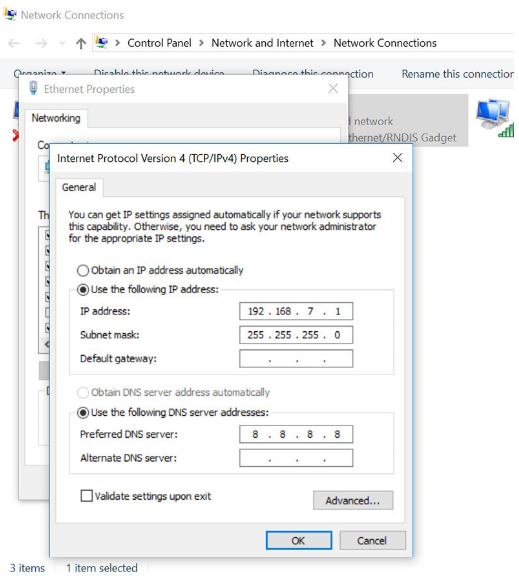
\includegraphics[width= 0.4\textwidth]{figs/img/Lab0/InternetGate_4.png}
 %   \caption{Setting IP Address Prompt}
  %  \label{fig:InternetGate_4}
%\end{figure}

%
%
%Finally, you should have noticed that the SSH connection has closed between the BeagleBone Black and your computer due to the network connection resetting. Just restart PuTTY and connect to the IP address 192.168.7.2 and login same as before. Now the internet is working but you still need to add a name server to translate the IP addresses into names and vice versa. textbf{To run the following command you must be the root user!} You can do this by typing the following command on the BeagleBone:
%     \begin{verbatim}
%        sudo su root
%
%        <if prompted, enter your password and confirm> 
%
%        echo "nameserver 8.8.8.8" >> /etc/resolv.conf
%
%        su debian
%     \end{verbatim}
%
%This command adds the google name server IP address to the config file. You can now test the internet connection using a simple ping test to a web URL such as google.com:
%     \begin{verbatim}
%        ping google.com
%     \end{verbatim}
%
%You should receive a positive response from the web URL server. Now that you are connected to the internet you can run updates and install any software as required.

%If you are having trouble following these instructions, please see %the link in the footnote. %\footnote{\url{https://www.digikey.com/en/maker/blogs/how-to-conne%ct-a-beaglebone-black-to-the-internet-using-usb/cdf66181b3a5436e9a%d730e4ed4cf9ee}} Additional help may be found in the %Troubleshooting section on page 15.


%===========================================================================================================
%https://www.digikey.com/en/maker/blogs/how-to-connect-a-beaglebone-black-to-the-internet-using-usb/cdf66181b3a5436e9ad730e4ed4cf9ee
%==========================================================================================================

%\subsection{Install Text Editors}
%\label{sec:install-text-editors}
%There are several text editors that can be used to edit/write programs/files. The default text editor is \emph{nano} that is pre-installed when the debian OS is installed. A text file, test.txt can be opened and edited by simply typing the following command on the PuTTY console terminal.
%
%\begin{verbatim}
%nano test.txt 
%\end{verbatim}

%Emacs is another powerful text editor. This is recommended for expert linux users. This editor is not preinstalled. It can be installed using:
%
%\begin{verbatim}
%sudo apt-get install emacs 
%\end{verbatim}
%
%One can open the test.txt file using command: \emph{emacs test.txt}


\subsection{Software Installation}
\label{sec:softwareInstallation}
Once the board is connected to the internet make sure to run the following commands to update all software packages of the operating system. %
%
\begin{verbatim}
                       sudo apt-get update
                       sudo apt-get -y upgrade
\end{verbatim}
%
In addition, an open-source software for editing text will be installed. There are several software packages for a text editor that can be used to edit/write programs/files. The default software package for editing text (text editor) is \emph{nano} that is pre-installed when the debian OS is installed. A text file, \emph{test.txt} can then be opened and edited by simply typing the following command on the PuTTY console terminal. %
%
\begin{verbatim}
    nano test.txt 
\end{verbatim}
%
Emacs is another powerful text editor. This is recommended for expert linux users. This editor is not preinstalled. It can be installed using:
% sudo apt-get install emacs25 -y 
\begin{verbatim}
    sudo apt-get install emacs 
\end{verbatim}
%
One can open the test.txt file using the command on PuTTY console: 
\begin{verbatim}
    emacs test.txt
\end{verbatim}



\section{Running Your First Program}
\label{sec:firstprogram}

This section is dedicated to detail on how to run a program written in C programming language on to BBBlue single-board computer. For that, make sure that the package ``librobotcontrol", which contains C library programs for a \ul{robot control project.} The library functions defined in this package will be used to program BBBlue hardware. 
\subsection{Library Functions Setup}
Fortunately, the latest Debian OS image comes with the \emph{librobotcontrol} library package preinstalled. Therefore, there is no need to install this package separately. However, you will need to reconfigure \emph{librobotcontrol} package to set the device tree and configure which program to run automatically when you boot BBBlue\footnote{See \url{http://strawsondesign.com/docs/librobotcontrol/installation.html} for details.}. The steps to reconfigure the the \emph{librobotcontrol} package are given below. 

\begin{enumerate}[a)]
    \item Open PuTTY and enter hostname as ``192.168.7.2" and port as ``22" as shown in Figure~\ref{fig:PuTTYLog}. %
    %
    \begin{figure}
        \centering
        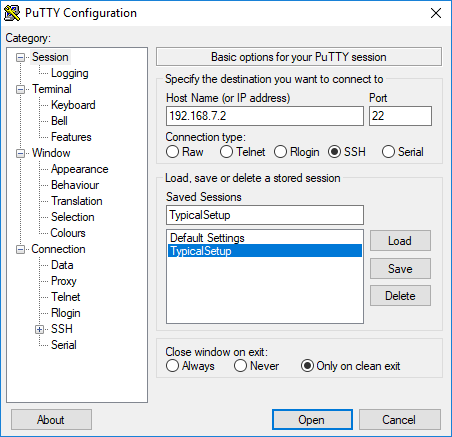
\includegraphics[width= 0.55\textwidth]{figs/img/Lab0/PuTTY.png}
        \caption{PuTTY Configuration Menu}
        \label{fig:PuTTYLog}
    \end{figure}    
    %
    At the configuration menu you will be presented with the options of Loading, Saving or Deleting a stored session. 
    Type ``Typical Setup" into the Saved Sessions box, then hit Save. Now click open. This will take you into the PuTTY console shown in Figure~\ref{fig:PuTTYcons}. If you saved the session, PuTTY will remember your hostname settings.
    
    
    \item Now you are in the PuTTY console. Login as ``debian" with the default password of ``temppwd". Now you are inside the BeagleBone. It will prompt you like the one shown in Figure~\ref{fig:PuTTYcons}. %
%
    \begin{figure}[H]
        \centering
        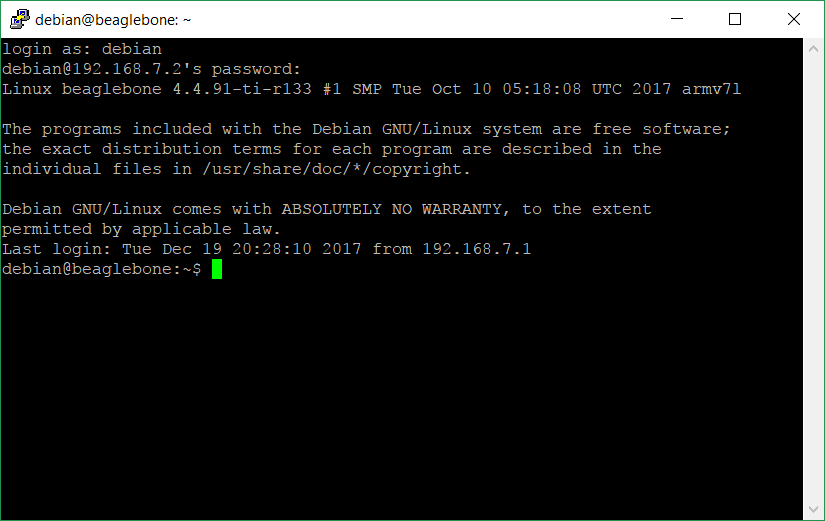
\includegraphics[width= 0.6\textwidth]{figs/img/Lab0/PuTTY_Console.png}
        \caption{PuTTY shell.}
        \label{fig:PuTTYcons}
    \end{figure}
    %
    \item  Check your default directory location by pressing ``pwd". It should read \emph{/home/debian}. If you are not in the correct directory then you will need to navigate through the file structure. Enter``ls" to check what folders you are able to navigate to. The only options available to you should be \textbf{bin}. You can create your own directory (or folder) by typing 
    \begin{verbatim}
        mkdir mechatronicsLabs
    \end{verbatim}
%    
      Hit \emph{Enter}, then type %
\begin{verbatim}
     cd mechatronicsLabs
\end{verbatim}
%
      to navigate to that folder.
    
    \item On the PuTTY terminal and run the following commands (one command at a time):
    
    \begin{verbatim}
        sudo dpkg-reconfigure librobotcontrol
        sudo apt update  && sudo apt upgrade librobotcontrol
    \end{verbatim}
    While these commands are executed, you may see the option which program to run automatically on boot. You may want to choose \underline{\emph{rc\_blink}} and then hit \emph{Enter} key. 
    \item Check that the librobotcontrol package is working properly by running the command: %
%    
    \begin{verbatim}
        rc_test_drivers
    \end{verbatim}
    You should see a window like the one shown in Figure~\ref{fig:rcTestDriver}.
    \begin{figure}
        \centering
        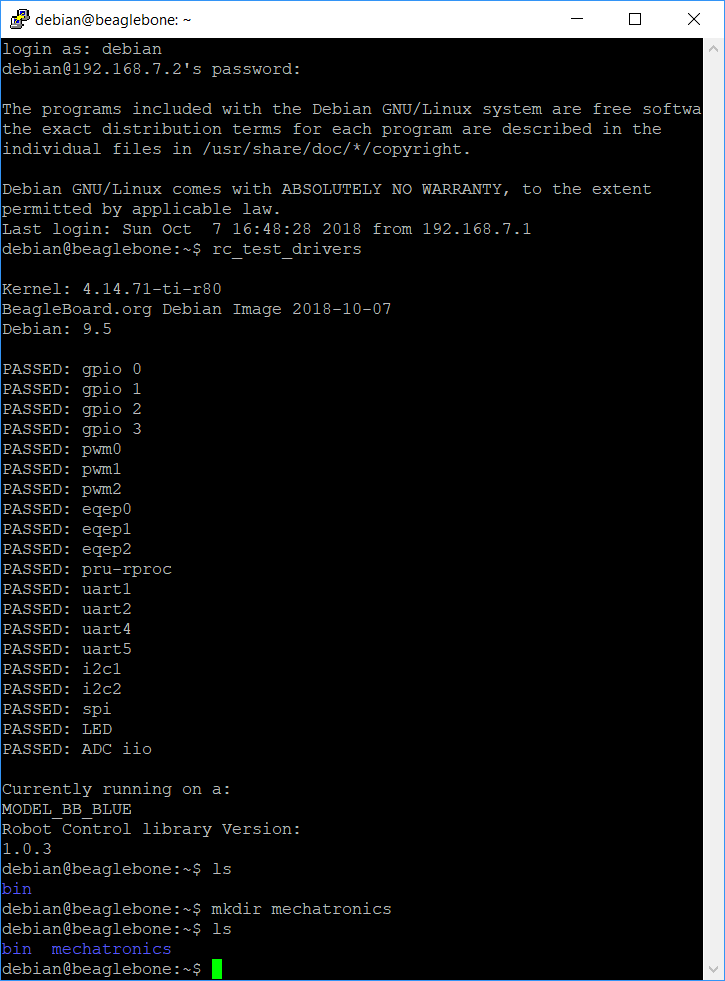
\includegraphics{figs/img/Lab0/rcTestDriver}
        \caption{Output of command \emph{rc\_test\_drivers}.}
        \label{fig:rcTestDriver}
    \end{figure}
    \item Check version of rc\_version program by typing
    \begin{verbatim}
         rc_version
    \end{verbatim}
    
    \end{enumerate}
    
    \subsection{Running C Program on BBBlue}        
    The main steps to run an existing C program (\emph{rc\_project\_template.c}) that is placed under the existing project template folder (\emph{rc\_project\_template}) are given below. 
    
    \begin{enumerate}
    \item On the PuTTY console window, run the following commands to make copy of the project template in your current directory, which is \emph{mechatronicsLabs}. %
    \begin{verbatim}
    cp -r /usr/share/robotcontrol/rc_project_template newProjectName
    cd newProjectName
    ls 
    \end{verbatim}
%
    \item Rename the current C program using 
    \begin{verbatim}
        mv rc_project_template.c exampleProgram.c 
        ls
    \end{verbatim}
    \item Edit the \emph{Makefile} using nano editor:
    \begin{verbatim}
        nano Makefile
    \end{verbatim}
    \item Replace the line \emph{TARGET = rc\_project\_template} with \underline{\emph{TARGET = newProjectName}}
    
    \item Compile the program using the command
    \begin{verbatim}
        make 
    \end{verbatim}
    \item Make sure that \emph{rc\_blink} program is not running on the BBBlue. If the \emph{rc\_blink} is running, then press and hold the \emph{PAU} button for four seconds. 
    
    \item Run the program in the BBBlue by typing the command
    \begin{verbatim}
        ./newProjectName 
    \end{verbatim}

\end{enumerate}

\section{Troubleshooting}
\label{sec:troubleshooting}
This section presents a partial list of issues that might appear while configuring a BBBlue for the first time. For convenience, a possible solution for each of these issues is given below.  
\begin{enumerate}[\emph{T\#}1:]
  
%\item After changing the ``Sharing'' option: Home networking connection to ``Ethernet 7'' http://192.168.7.2 will not work. Complete the network settings and then restart PuTTY session as before. Then, you will be able to connect to the board. 

  
%\item If BBBlue is booted (not booted) from SD card, the Ethernet adapter shows:  \emph{Ethernet 7, Remote NDIS Compatible Device \#2} (\emph{Ethernet 7,... Linux USB Ethernet/RNDIS}).
  
%\item If an error occurs when sharing networks, where the IP Address is automatically changed, refer to the \url{http://beagleboard.org/getting-started}
    
\item After installing the drivers, browsing http://192.168.7.2 doesn't work, \textit{i.e.,} BBBlue is not connected. \label{trst:problem2}
   
    \textbf{Solution:} Restart your computer and browse http://192.168.7.2 and it should show ``connected''

% \item Problem: After changing the ``Sharing'' option: Home networking connection to ``Ethernet 7'' http://192.168.7.2 will not work. \label{trst:problem3}

%     \textbf{Solution of~\ref{trst:problem3}:}  Complete the network settings and then restart PuTTY session as before. Then, you will be able to connect to the board.  
    
\item \emph{sudo apt-get -y upgrade}  automatically installs robotics cape library and asks which program to run when the board boots. \label{trst:problem4}

    \textbf{Solution:}  $\Rightarrow$ choose \emph{rc\_blink}
    
\item Abnormal issues concerning network connection, commands, and any other issues. \label{trst:problem1}
    
    \textbf{Solution:}  Re-flashing the SD card should resolve any abnormality.

    
  \item There may be some issues caused by not turning off the BBBlue properly. Therefore, use the following command to safely shutdown the Beaglebone when you are done working with it.

\begin{verbatim}
sudo shutdown now
\end{verbatim}
    If this command is not run, there is a chance that the Beaglebone's flash memory will be corrupted. Therefore it is very important that you run this command to turn off the board instead of simply pulling out the USB power cable.

\end{enumerate}

\section{Useful Links}
\label{sec:useful-links}

Some weblinks that are useful for BBBlue are listed below. 

\begin{enumerate}
\item \href{http://wiki.seeedstudio.com/BeagleBone_Blue/}{http://wiki.seeedstudio.com/BeagleBone\_Blue/}
  
\item \href{https://beagleboard.org/blue}{https://beagleboard.org/blue}
  
\item \href{http://strawsondesign.com/docs/librobotcontrol/index.html}{http://strawsondesign.com/docs/librobotcontrol/index.html}
  
\item \href{https://www.renaissancerobotics.com/BeagleboneBlue.html}{https://www.renaissancerobotics.com/BeagleboneBlue.html}
\end{enumerate}



%%% Local Variables:
%%% mode: latex
%%% TeX-master: "../../mainDocument"
%%% End:

 

\bibliographystyle{plain}
\bibliography{bib/refsBooksTRTheses}

\end{document}

%%% Local Variables:
%%% mode: latex
%%% TeX-master: t
%%% End:




%%% Local Variables:
%%% mode: latex
%%% TeX-master: t
%%% End:
